\documentclass[a4paper,12pt]{report}

\usepackage[T2A]{fontenc}
\usepackage[utf8]{inputenc}
\usepackage[english,ukrainian]{babel}
\usepackage{amsmath}
\usepackage{ragged2e}
\usepackage{graphicx}
\usepackage{listings}
\graphicspath{ {./} }

\usepackage{titlesec}
\titleformat{\section}[block]{\Large\bfseries\filcenter}{}{1em}{}
\titleformat{\subsection}[block]{\bfseries\filcenter}{}{1em}{}

\author{Кирило Байбула Аленович}
\title{Визначення швидкодії обчислювальної системи}
\lstset{frame=tb,
  language=C,
  aboveskip=3mm,
  belowskip=3mm,
  showstringspaces=false,
  columns=flexible,
  basicstyle={\small\ttfamily},
  numbers=none,
  numberstyle=\tiny\color{gray},
  breaklines=true,
  breakatwhitespace=true,
  tabsize=3
}


\begin{document}

\begin{titlepage}
	\begin{center}
		\Large
		\textbf{Київський національний університет імені Т.Шевченка}
		\vspace{5cm}

		\Huge
		\textbf{Звіт}

		\LARGE
		До лабораторної роботи №1
		\vspace{0.5cm}

		\textbf{ВИЗНАЧЕННЯ ШВИДКОДІЇ ОБЧИСЛЮВАЛЬНОЇ СИСТЕМИ}
		\vfill
	\end{center}

	\begin{FlushRight}
		Кирило Байбула Аленович\\
		Групa К-21\\
		Факультету комп’ютерних наук \\
		та кібернетики
	\end{FlushRight}

	\vspace{0.5cm}

	\begin{center}
		\textbf{Київ} \\
		2021
	\end{center}

\end{titlepage}
\clearpage

\section{МЕТА}
Метою даної лабораторної роботи є розробка програми, яка б вимірювала кількість виконуваних базових операцій за секунду конкретною \textbf{Обчислювальною Системою} (комп’ютер + ОС + Система програмування та мова програмування). Лабораторна робота не передбачає вимірювання \textit{“чистої”} команди процесора. Розроблена програма має бути зібрана та запущена у \textbf{віртуальній машині} або \textbf{контейнері}. Вибір системи програмування, комп’ютера та ОС не є регламентованим. Результати повинні бути представлені у табличній формі з відображенням для кожного тесту:
\begin{enumerate}
    \item{Назви команди/операції;}
    \item{Типу/формату даних;}
    \item{Кількості операцій за секунду;}
    \item{Лінійної діаграми значення швидкості у відсотках відносно найшвидшої команди/операції, яка береться за 100 \%}
    \item{Значення у відсотках.}
\end{enumerate}

\section{МЕТОД ОБЧИСЛЕНЬ}

Для цієї лабораторної роботи за систему програмування були взяті мова програмування Сі та операційна система GNU\textbackslash Linux в частності дистрибутив Pop\_OS!, що стоїть на домашньому лєптопі з процессором Intel i5-8250U з тактовою частотою 3.400GHz. Також далі для віртуальної операційної буде задіян Docker контейнер з докер-образом операційної системи Alpine Linux. Для вимірювань у мові програмування Сі будуть використовуватися найпростіші базові операції, такі як: додавання, віднімання, множнення та ділення, які будуть виконуватися над типами \textit{char, int, long, float} та \textit{double}. Для вимірювання часу виконання коду буде підключен загаловочний файл \textbf{<time.h>}, що має потрібні нам фунцію \textbf{clock()} та конcтанту \textbf{CLOCKS\_PER\_SEC}. Для отримання фактичного часу виконання операції необхідно було відняти від зафіксованого для даної операції часу, час “порожнього циклу” та час виконання усіх операцій присвоювання, а далі розділити отримане значення  на кількість виконань цієї операції.  Пам’ятаючи, що бажаним для нас результатом є кількість операцій за секунду, то кінцевий результат знаходився, як одиниця розділена на фактичний час виконання операції.

\section{ОБЧИСЛЮВАЛЬНА СИСТЕМА}
\begin{itemize}
  \item{Процесор:Intel® i5-8250 CPU @ 3.400GHz}
  \item{Операційна система: GNU\textbackslash Linux}
  \item{Система програмування: Emacs 28, компілятор GCC, дебаггер GDB}
  \item{Програма контейнерізації для операційних систем: Docker}
\end{itemize}

\section{РЕЗУЛЬТАТ РОБОТИ ПРОГРАМИ}
\subsection{Власна обчислювальна система}
\begin{center}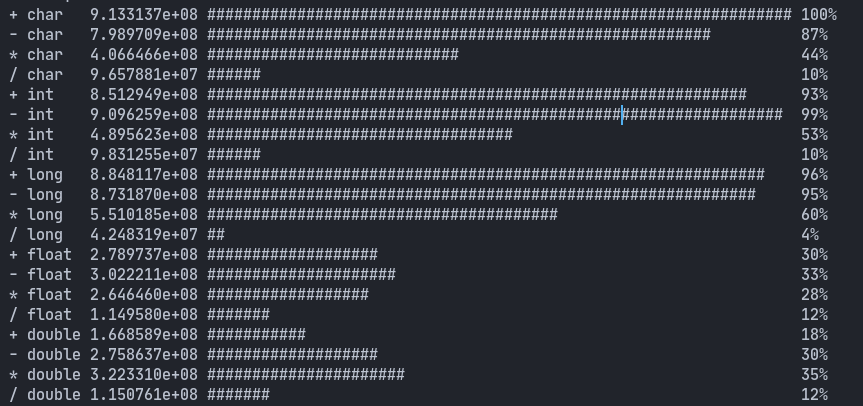
\includegraphics[scale=0.4]{main}\end{center}
\subsection{Віртуальна обчислювальна система} \begin{center}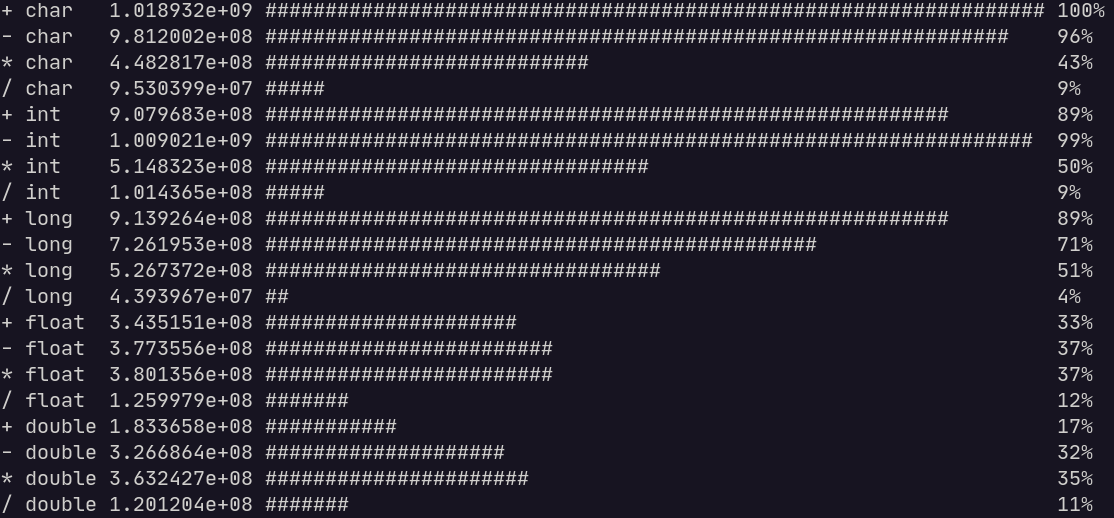
\includegraphics[scale=0.4]{vir}\end{center}

\section{Висновок}
Задача порівняння ОбСист стає досить актуальною для сучасного ринку інформаційних технологій (ІТ), прикметною рисою якого є швидке моральне старіння всієї інфраструктури ІТ. Ринок ІТ починає тиснути на користувача в плані нових витрат, які часто є реакцією на вдало проведені маркетингові акції, а не фактичною потребою таких витрат. Врешті, навіть невеликі витрати на кожний комп’ютер компанії в рамках сотень і тисяч робочих місць у останній може потребувати значні кошти. Сама ж ІТ-індустрія не задовольняється тим, що ряд систем, пристроїв можуть довго використовуватися, - все вироблене має розкуповуватися вже сьогодні, і нас виробники мусять переконувати робити постійну, власне часто зайву для вас, модернізацію всього. В цій ситуації для користувача – від домашнього до корпоративного – важливо мати деякий якісний орієнтир реального виграшу чи його відсутності.

\end{document}
